\begin{table} 
\begin{center} 
\begin{tabular}{|c||c|c|c|c|}
\hline
\emph{Algorithm} & \emph{Manifold Model} & \emph{Encode} & \emph{Decode} & \emph{Relate Enc. \& Dec.}\\
%\thickhline
\hline \hline 
\cellcolor{red}PCA & Linear &\checkmark & \checkmark & $W_D = W_E ^T$\\
\hline
\cellcolor{red}ICA & Linear &\checkmark & \checkmark & $W_D = W_E ^T$\\
\hline
\cellcolor{yellow}Sparse Coding & Local Linear &\checkmark & \checkmark & Separate \\
\hline 
\cellcolor{yellow}CBP & Osculating Circle &\checkmark & \checkmark & Separate \\
\hline 
\cellcolor{yellow}PSD \& LISTA & Local Linear &\checkmark & \checkmark & Separate\\
\hline
\cellcolor{lightblue}DrLIM & Nonlinear & \checkmark & X & Enc. Only\\
\hline
\cellcolor{lightblue}Chapter \ref{chapter:slow} & Nonlinear & \checkmark & X & Enc. Only\\
\hline
\cellcolor{lightblue}Chapter \ref{chapter:linear} & Nonlinear & \checkmark & \checkmark & Separate\\
\hline
Adversarial Networks & Nonlinear & X & \checkmark & Dec. Only \\
\hline 
\cellcolor{green}Auto-Encoders & Nonlinear & \checkmark & \checkmark & Separate \\
\hline 
\end{tabular} \\
\vspace{0.25cm} \hspace{0.25cm}  
\begin{tabular}{|c|}
\hline 
\emph{Model Objective/Prior}\\  
\hline \hline
\cellcolor{red} De-correlation/Independence  \\
\hline
\cellcolor{yellow} Sparsity \\
\hline
\cellcolor{lightblue} Metric Learning/Geometric Prior  \\
\hline
\cellcolor{green} All of the Above \\
\hline
None \\
\hline
\end{tabular}
\end{center}
\caption{Summary of unsupervised feature learning algorithms and their properties} 
\label{tbl:models} 
\end{table} 

Unsupervised feature learning arguably dates back to the invention of Principal
Component Analysis (PCA) in 1901 by Karl Pearson \cite{PCA}. As mentioned in
Chapter \ref{chapter:introduction}, feature learning algorithms model
intrinsically low dimensional data embedded in a high dimensional ambient
space. These models can usually be decomposed into two parts: a mapping from
the input space to the feature space, called encoding, and mapping the feature
space back to the input space, called decoding. If the encoding or decoding
processes have corresponding functional forms, they are referred to as the
``encoder'' and ``decoder'', respectively.  From the natural image manifold
perspective, ideal encodings map the extrinsic coordinates (i.e. pixel values)
to intrinsic manifold coordinates. It is hoped that these intrinsic coordinates
correspond to physical attributes of the natural world, such as the presence of
certain objects in the scene, their properties, etc \cite{nair2008,capsules}.
Unsupervised feature learning models are mainly distinguished by: (i)-whether
they assume a deterministic or probabilistic model, (ii)-the geometrical prior
they assume about the data manifold, (iii)-whether they learn an encoder,
decoder, or both. For example, Principal Component Analysis assumes that the
data is concentrated around a hyper-plane, i.e. it assumes a globally linear
data manifold model. The PCA encoder is a matrix operator, $W_e$, as is the
decoder $W_d=W_e^T$. Although probabilistic models is not the focus of this
work, we will see a connection between probabilistic and deterministic models
in Chapter \ref{chapter:SATAE}.  Obtaining ``invariant'' representations has
been a major driving force in feature learning, driven mainly by recognition
and classification problems.  Invariant features imply that the encoding
process is necessarily a many-to-one mapping. This means that the decoding
process must involve some random selection among the possible inputs that
produced the code, usually  by sampling from a distribution. Models that
include a decoder are called ``generative models'' in the literature. 

Table \ref{tbl:models} summarizes key aspects of several well-known feature
learning models, as well as the new models which will be introduced in Chapters
\ref{chapter:slow} and \ref{chapter:linear}. The first column lists the name of
the model, the color indicates the type of objective each model tries to
optimize. For example, one version of PCA finds maximally decorrelated linear
components. The ``manifold model'' column indicates the geometric prior each
model assumes about the data manifold. As another exampling,  the Continous
Basis Pursuit (CBP) model proposes a local osculating circle model to the data
manifold \cite{CBP}.  The next two columns indicate whether each model learns
an encoder and/or decoder.  Finally, the last column summarizes the
relationship enforced between the encoder and decoder. For example in PCA the
encoder and decoder are related by the transpose operator. This chapter will
review some of the algorithms in Table \ref{tbl:models}, placing emphasis on
the precursors of the algorithms presented in Chapters \ref{chapter:slow} and
\ref{chapter:linear}. The algorithms will be presented as various models of the
data manifold.

\section{Principal and Independent Component Analysis} 

\begin{figure} 
\centering
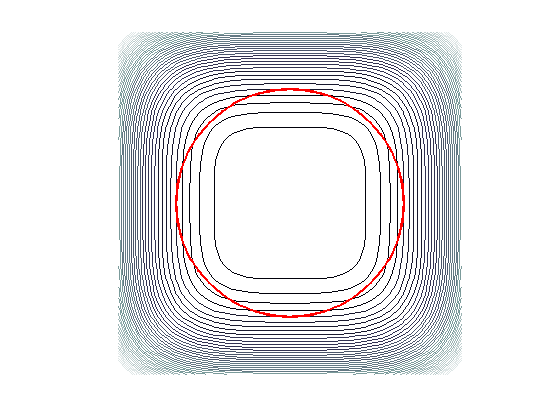
\includegraphics[scale=0.4]{./figures/related_work/ICA.png} 
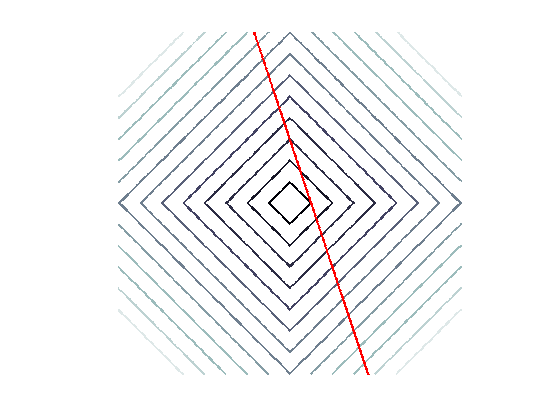
\includegraphics[scale=0.4]{./figures/related_work/L1.png} 
\caption{Left: visualization of the optimization problem used to solve for independent representations. Right: visualization of the optimization problem used to solve for sparse representations.} 
\label{fig:ICA_lasso} 
\end{figure}  

Principal Component Analysis (PCA) and Independent Component Analysis (ICA) are
the most well know linear manifold models \cite{ICA}. Both assume that the
observed high dimensional data $x$ are generated from some low dimensional
latent variables $z$ via a linear operator $A$, that is $x=Az$. Assuming that
the data is zero mean, PCA implicitly makes the assumption that the latent
variables correspond to directions with the largest variance \cite{PCA}.  These
components can be obtained from the Eigen decomposition of the covariance
matrix.  ICA however searches for linearly independent components, formulating
the definition of independence using the central limit theorem. Although the
detailed derivation of ICA will not be presented here, we will mention that it
leads to a fourth order moment (kurtosis) maximization problem subject to a
second order moment (variance) constraint. This optimization problem is
visualized as the left plot of Figure \ref{fig:ICA_lasso}. The blue curves
represent the level sets of the kurtosis objective, and the red curve
represents the unit variance constraint. Figure \ref{fig:ICA_features}  shows
the features learned using an ICA algorithm on natural image patches.  Note the
strong resemblance to the bases learned with sparse feature learning algorithms
such as Sparse Coding \cite{SC}. The next section will establish a
connection between ICA and sparse inference.  

\begin{figure} 
\centering
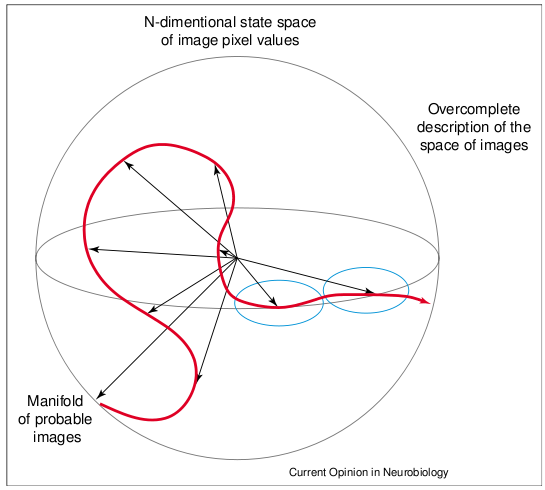
\includegraphics[scale=0.4]{./figures/related_work/imageManifold.png} 
\caption{Sparse coding learns a local linear model of the data manifold (source: \cite{SC2}).}
\label{fig:ICA_features} 
\end{figure} 

\begin{figure} 
\centering
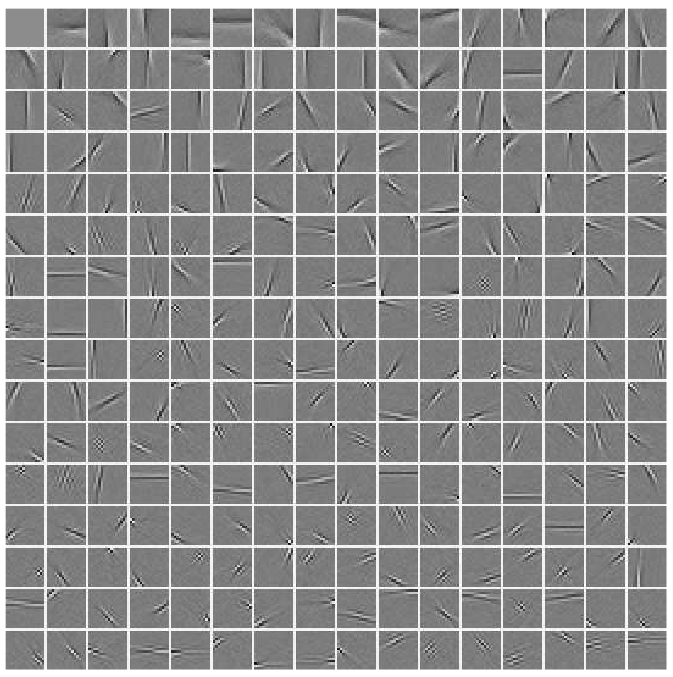
\includegraphics[scale=0.4]{./figures/related_work/ICABasis.png} 
\caption{Independent features learned on natural image patches (source: \cite{ICA}).}
\label{fig:ICA_features} 
\end{figure} 

\section{Sparse Representations} 
Sparse inference refers to the problem of finding the sparse coefficients $z$ which
reconstruct the input $x$ as a linear combination of some basis elements
contained an over-complete dictionary $W_d$. Sparsity is measured by the number
of non-zero coefficients; the higher the sparsity the fewer non-zero
coefficients in $z$ used to represent $x$.  
The sparse inference problem can be stated formally as: 

\begin{equation} 
\min \|z\|_0 \mbox{ subject to } x = W_dz 
\end{equation} 

In general, this is an intractable combinatorial problem. A now famous
breakthrough showed that exact sparse solutions can be obtained, under certain
conditions, by replacing the $L_0$ norm with an $L_1$ norm \cite{candes2006}.
This optimization problem is depicted on the right side of Figure
\ref{fig:ICA_lasso}.  The level sets of the $L_1$ norm are shown in blue and
the linear constraint is shown in red. The minimum occur on the $x$-axis, with
$y=0$ implying that the solution is indeed sparse. Remarkably, the solution to
the ICA problem (left side of Figure \ref{fig:ICA_lasso}) is also sparse though the
objective was explicitly not derived with sparsity in mind. Given this similarity 
between ICA and sparse feature learning, it is not surprising that the features 
learned with ICA on natural images strongly resemble those learned with sparse coding. 

Relaxing the constraint, this problem can be written as an unconstrained loss
functional called the lasso (also basis pursuit de-noising) \cite{BP}:  

\begin{equation} 
L_{lasso} = \frac{1}{2}\|x-W_dz\|^2_2 + \alpha \|z\|_1
\label{eqn:lasso} 
\end{equation} 

Minimizing the above loss with respect to $z$ and a fixed $W_d$ corresponds to
the sparse inference problem, which also corresponds to the ``encoding''
process. Decoding sparse representations is trivial, it simply corresponds to
computing $W_dz$.  The loss described by the above equation is non-convex with
respect to $z$, however each of the two terms are individually convex which
prompted alternating minimization approaches such as the various Iterative
Shrinkage and Thresholding algorithms \cite{FISTA}. It is possible to find a
``feed forward'', i.e. non-iterative approximation (i.e. encoder) to
iterative sparse inference algorithms for data $x$ drawn from a stationary
distribution. Thus the coefficients are given by a functional mapping of the input,
i.e. $z=F_W(x)$. This mapping, called the encoder, can be learned jointly with
the decoder.  The corresponding loss is given by Equation \ref{eqn:sae_loss}, 

\begin{equation} 
L_{SAE} = \frac{1}{2}\|x-W_dF_W(x)\|^2_2 + \alpha \|F_W(x)\|_1
\label{eqn:sae_loss} 
\end{equation} 

The above loss can be implemented using a network architecture called an
``auto-encoder''. Depending on the functional form of $F_W$, the above loss can
be highly non-convex with no known optimal minimization algorithm,
however stochastic gradient descent works well in practice.  Because of the
sparsity-inducing $L^1$ penalty on the coefficients, this is called the sparse
auto-encoder (SAE) \cite{SAE1,SAE2}. Optimal architectures for $F_W()$ in the
SAE network are the subject of Chapter \ref{chapter:LISTA}. Other auto-encoder
networks will be discussed later in this chapter.    
\newline 
\indent  
It was noticed that when sparse feature learning was applied to natural images,
local edge detectors similar to the Gabor wavelet basis emerged. Gabor wavelets
were already being used in many computer vision applications \cite{SC,gabor}.
This observation lead to a flurry of works that tried to apply sparse features
to common computer vision problems such as object detection and recognition.
One problem with sparse representations is their instability. A sparse code
corresponding to an overcomplete basis implies that each basis element is
selective and is activated only be specific inputs; an edge at a specific
location and orientation for example. If the edge moves slightly, a different
basis element will respond, corresponding to a change of support in code space.
This highly unstable behavior of sparse representations is undesirable for
tasks such as classification where \emph{invariance} is an important property.
For example, the object category remains the same under many transformations.
One way to mitigate this behavior is to combine the responses of several basis
elements such that the response of the group is more stable than the response
of the individual elements.  This so called ``group sparsity'' results in
feature representations that are much more stable and hence more useful for
tasks that require invariant representations \cite{groupSparsity, ICA, yuan2006model}. 
Groups of feature activations can be combined using so called ``pooling''
operators, which partition the activations into groups and typically output
their $L^2$ norm.  In group-sparse models, the sparsity inducing $L^1$ norm is
applied to the grouped activations, i.e. to the output of the local $L^2$
pooling operator.  Specifically, if the code space is partitioned into $K$
potentially overlapping neighborhoods, where $P_i$ denotes the $i^{th}$
neighborhood, the group sparsity loss can be written as: 

\begin{equation} 
L_{GSC} = \frac{1}{2} \|x - Wz \|_2 ^ 2 + \alpha \sum_{i=1} ^ K \sqrt{\sum_{j \in P_i} w_jz_j ^2}  
\label{eqn:gsc_loss} 
\end{equation}

Note that if the optional neighborhood weights $w_j$ are all set to unity, the
second term reduces to a sum of $L^2$ norms.  The features learned with this
model are shown in Figure \ref{fig:GSC_features}.  Note that the local
overlapping pooling operator introduces a global topology in the feature space,
whereby nearby features tend to co-activate. The models presented in Chapters
\ref{chapter:slow} and \ref{chapter:linear} extend this idea to temporal data
in order to learn feature groups that correspond to temporal transformations.    

\begin{figure} 
\centering
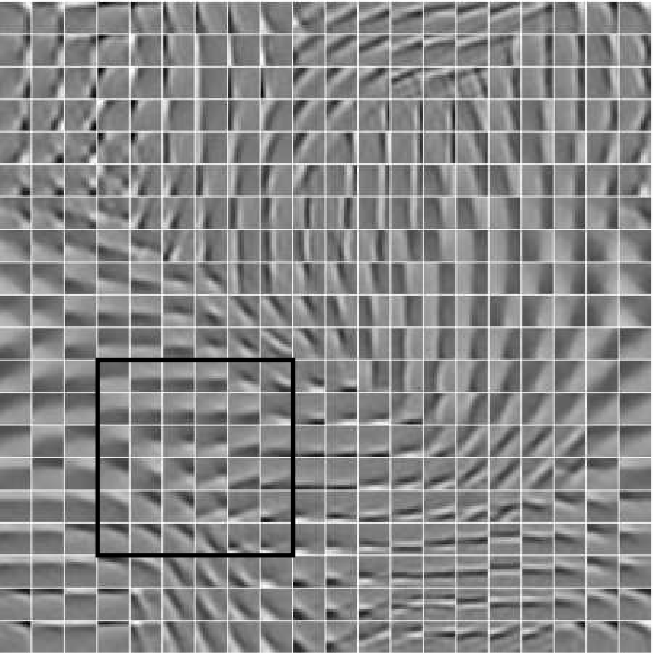
\includegraphics[scale=0.4]{./figures/related_work/PSD.png} 
\caption{Features learned with group sparsity model in a two dimensional topology, 
with a local pooling neighborhood is overlaid in black. Figure from \cite{groupSparsity}.}
\label{fig:GSC_features} 
\end{figure} 
 
\section{Auto-Encoders and Energy Based Learning} 

An auto-encoder is a conceptually simple neural network used for obtaining
useful data representations through unsupervised training. Where the usefulness
is usually measured by applying them to some other task, such as
classification.  This network is composed of an encoder which outputs a hidden
(or latent) representation and a decoder which attempts to reconstruct the
input using the hidden representation as its input.  Training consists of
minimizing a reconstruction cost such as $L_2$ error.  However this cost is
merely a proxy for the true objective: to obtain a useful latent
representation. Auto-encoders can implement many dimensionality reduction
techniques such as PCA and Sparse Coding \cite{DHS,SC,LISTA}.
This makes the study of auto-encoders very appealing from a theoretical
standpoint. In recent years, renewed interest in auto-encoders networks has
mainly been due to their empirical success in unsupervised feature learning
\cite{SAE1,SAE2,CAE,DAE}. 

In the previous subsection we have seen that sparse coding has a corresponding
auto-encoder network implementation. In the sparse auto-encoder, a
sparsity-inducing $L^1$ penalty is applied to the code, i.e. output of the
encoder. Other penalties are possible and impose different priors on the
representation. In general these architectures are called regularized
auto-encoders. In this subsection we will briefly mention several important
regularizers, and introduce a new regularizer in Chapter \ref{chapter:SATAE},
where auto-encoders are discussed in more detail. With appropriate regularization,
auto-encoders embody an implicit model of the data manifold. The reconstruction
error for a sample that is near the manifold should be low and high for points not
near the data manifold.  In the following chapter we argue that the role of the
regularizer is to ensure that reconstruction error (energy) is large for points
far from the data manifold. In this sense the reconstruction energy can be seen
as an unnormalized inverse probability of a sample belonging to the data generating
distribution \cite{lecun2006}. Two popular regularized auto-encoder models
include the Contractive Auto-Encoder (CAE) and the De-noising Auto-Encoder
(DAE) \cite{CAE,DAE}. Both can be interpreted as implicit models of the data
manifold. The DAE is trained to reconstruct input samples from their 
corrupted versions. The corruption process usually involves setting a random subset 
of the input dimensions to zero. This forces the model to infer the original uncorrupted pixels 
values from neighboring pixels. One interpretation of the DAE is that it projects 
corrupted samples to their nearest uncorrupted counterparts on the data manifold. The
contractive auto-encoder introduced an explicit penalty on the Frobenius 
norm of the Jacobian of the code with respect to the input. The loss corresponding 
to the contractive auto-encoder is: 

\begin{equation} 
\nonumber 
L_{CAE} = \frac{1}{2} \|x - Wz \|_2 ^ 2 + \alpha \sum_{ij} \left(\frac{\partial z_i}{\partial x_j}\right)^2  
\end{equation}  

Where $z_i$ and $x_j$ denote the $i^{th}$ component of $z$ and $j^{th}$
component of $x$, respectively.  The second term in the loss encourages a
stable, or invariant, representation $z$. However $z$ cannot be perfectly
stable since it must be informative enough to reconstruct the input. From the
manifold perspective, the mapping learned by the encoder is mainly allowed to
vary in the principal directions of the data manifold.           

\section{Metric Learning}
Another important class of machine learning problems from which useful features
can be learned are the metric or similarity learning problems
\cite{tenenbaum2000,DrLIM}. Metric learning problems aim to learn a feature
space which satisfies certain metric properties given by (weakly) labeled data.
For example we may wish to find a feature space in which images of objects that
belong to the same category are closer to each another than objects from
different categories. Many metric learning algorithms define a graph on the
data whereby ``similar'' samples are connected by an edge, and the metric
between samples are given by geodesics (shortest paths) on this graph structure
\cite{tenenbaum2000, coifman2006}. Most classical metric learning algorithms,
however, suffer from the so called ``out of sample extension'' problem
\cite{bengio2004out,coifman2006geometric}. The problem is related to new samples 
introduced at test time; new samples potentially change the adjacency graph 
unpredictably which in turn requires re-running the geodesic computation every
time a new sample is introduced. One solution to this problem is to train an
encoder that projects the data into feature space with the desired metric
properties. One method that does this is known as Dimensionality Reduction by
Learning an Invariant Mapping \cite{DrLIM}. The encoder mapping, $G_W()$ is
trained by stochastically optimizing the metric relationship between pairs of
points, $\{x_i$,$x_j\}$.  If the points are deemed similar via some (weak)
label ($Y=0$) then their distance is encouraged to decrease. Conversely if they
are dissimilar, with label $Y=1$, their distance is encouraged to increase to
at least some margin value $m$. This acts as a contrastive term and prevents 
the mapping $G_W()$ from collapsing and producing constant outputs. These two 
terms are combined to form the following loss:            
\begin{equation} 
L(W,Y,X_1,X_2) = (1-Y)\frac{1}{2}\|G_W(x_i)-G_W(x_j)\|^2 + Y \frac{1}{2}\max(0,m-\|G_W(x_i)-G_W(x_j)\|^2)  
\end{equation}  
Unfortunately, as we will also show that the second term is a very weak
requirement in high dimensional feature spaces and can be trivially 
optimized. 
\section{Summary} 
Assuming that natural data lies on a low dimensional manifold, is perhaps a
necessary but not sufficient condition for specifying a complete model of the
data, and learning useful features.  Other characteristics of the data must be
assumed to obtain not only necessary but sufficient conditions for for
obtaining a useful characterization of the data. Often this includes
characterizing the process by which the data was generated
\cite{bishop2006pattern,blei2003latent}.   The modus operandi of unsupervised
feature learning research is to guess what the generic characteristics of
natural data are, and then to derive the corresponding losses and architectures
that maximize these properties; of which sparsity, slowness, 
and independence are just a few popular examples.      
